\section{Stochastic Emission at Small Angular Scales} \label{sec:small_scales} 

% Susan editing/commenting 4/19
\subsection{Methodology}\label{subsec:methodology}
The methods presented here aim to preserve the well-measured large-scale information in our various templates, filter out the noisy small-scale emission in those templates, and replace those small scales with a stochastic realization that has a reasonable correspondence with the large scale emission. Specifically, the synthetic small-scale structure should have a power spectrum that connects smoothly to the power spectrum of the real data at large scales and should inherit some of the amplitude information from the large-scale data. Our approach is to construct small-scale stochastic templates and then modulate them with the large-scale amplitude data.

Rather than $I$, $Q$, and $U$, we choose to work with their analogues in the polarization fraction tensor framework (Frolov et al., in prep.). This provides a physically-motivated way to couple intensity and polarization self-consistently, and the nature of the logarithmic transformations introduces some non-Gaussianity into the final maps {\bf [see Section X]}. The transformations from $I$, $Q$, and $U$ to $i$, $q$, and $u$, respectively, are

\begin{align}
    i &\equiv \frac{1}{2} \ln (I^2 - P^2)\nonumber  \\
    q &\equiv  \frac{Q}{2P} \ln \frac{I+P}{I-P} \label{eq:pt2real}\\
    u &\equiv  \frac{U}{2P} \ln \frac{I+P}{I-P}\nonumber 
    ~~~,
\end{align}
where $P \equiv \sqrt{Q^2 + U^2}$.

The inverse transformations are:

\begin{align}
    I &= e^i \cosh p \nonumber \\
    Q &= \frac{q}{p}e^i\sinh p \label{eq:real2pt} \\
    U &= \frac{u}{p}e^i\sinh p \nonumber
    ~~~,\label{eq:real2pt}
\end{align}
where $p \equiv \sqrt{q^2 + u^2}$.

The method for generating small-scale emission can be summarized as follows: 
\begin{enumerate}
    \item We first transform the $I$, $Q$, and $U$ templates into the $i$, $q$, and $u$ maps via Equation~\eqref{eq:real2pt}. 
    \item We then compute the $tt$, $te$, $ee$, and $bb$ full-sky power spectra from the $i$, $q$, and $u$ maps in analogy with how $TT$, $TE$, $EE$, and $BB$ spectra are computed from $I$, $Q$, and $U$ maps. 
    \item We construct a simple model for each of the $tt$, $te$, $ee$, and $bb$ spectra by first estimating the amplitude of each power spectrum $A_{\ell, 1}$ at some pivot scale $\ell_1$ by fitting it with a power-law of fixed index, taken from the literature. We adopt the input templates as-is for $\ell < \ell_1$, extrapolate the spectrum with this power law from $\ell_1$ until a second pivot scale $\ell_2$, and then finally extrapolate to $\ell > \ell_2$ with the power law index of the $tt$ spectrum.
    \item We construct modulation maps $m_I$ and $m_P$ for intensity and polarization, respectively, following the methods in Section~\ref{subsec:modulation}.
    \item We then synthesize $i$, $q$, and $u$ maps using the constructed $tt$, $te$, $ee$, and $bb$ spectra. These maps are then high-pass filtered at cut-off multipole $\ell_1$ and multiplied by the modulation maps. 
    \item We low-pass filter the template $i$, $q$, and $u$ maps with cut-off multipole $\ell_1$. 
    \item Finally, we sum the small-scale and large-scale maps and then transform back to $I$, $Q$, and $U$ maps via Equation~\eqref{eq:pt2real}. 
\end{enumerate}

This prescription has several free parameters that require tuning. The pivot scale $\ell_1$ governs to which multipole information is taken from the input template maps versus what is generated randomly. The pivot scale $\ell_2$ prevents the $TE$, $EE$, or $BB$ spectra from exceeding the $TT$ spectrum at any scale. While such power spectra are not necessarily unphysical, maps synthesized from them can produce pixels with polarization fractions in excess of unity unless other constraints are imposed. Finally, the modulation maps $m_I$ and $m_P$ ensure that fluctuations are larger in bright regions (e.g., at low Galactic latitude) and smaller in faint regions (e.g., at high Galactic latitude).

All high- and low-pass filtering is done via the sigmoid function: 
\begin{equation}
\sigma (\ell; \ell_k, \Delta \ell ) = \left( 1+  \exp \left( - \frac{2 (\ell - \ell_k  +\Delta \ell ) }{\Delta \ell}\right)   \right)^{-1}.
\end{equation}
 

\begin{table*}[]
    \centering
    \footnotesize
    \begin{tabular}{lccccccc}
    \toprule 
   &   $ \ell_1  $&$\ell_2$   &$\ell_* $& $\alpha_{TT}$  & $\alpha_{EE}$ &$\alpha_{TE}$ &$\alpha_{BB}$ \\
   \midrule  
   Thermal dust & 100 & 2000 & 80 & -0.80$^2$ & -0.42$^{1}$& -0.50$^{1}$ & -0.54$^{1}$ \\ 
   Synchrotron & 38 & 400 & 36 &  -1.00& -0.84$^{1}$ & -1.00 & -0.76$^{1}$ \\
   \bottomrule
    \end{tabular}
    \caption{Spectral indices fit from the functional form,  $D_{\ell}\propto \ell^{\alpha}$, $^1$\citet{planck2016-l11A}, $^2$\citet{mivilledeschene:2016}}
    \label{tab:smallscale_par}
\end{table*}


%We estimate  the $tt$, $ee$, and $bb$  full sky power spectra from the $i$, $q$, and $u$ maps  just as $TT$, $EE$, and $BB$ spectra are computed from $I$, $Q$, and $U$ maps.  We fit each power spectrum with a power law in $\ell$ over a range of $\ell$ motivated by the resolution of the map. We use this power law fit, sometimes adjusted for physical considerations described below, as the basis for generating small-scale fluctuations. We construct a map of small scale fluctuations following the prescribed spectrum and then modulate these fluctuations by multiplying by a scaled version of the intensity map. This ensures that the amplitude of fluctuations in the Galactic plane are larger than those at high Galactic latitudes. Finally, we add the low-pass filtered $i$, $q$, and $u$ maps to the map of small-scale fluctuations and then transform back to $I$, $Q$, and $U$ to produce the final set of maps. {\bf would it be useful to introduce general equations in this section, e.g., how the large and small scales are joined with the sigmoid function?}

Since the generation of the small scales depends only upon a fixed input power spectrum, we can generate a different map realization on the fly each time a sky is simulated. Thus, the new PySM models presented here can provide an ensemble of realizations having the same well-measured large scales but random realizations of the poorly-measured small scales. Further, the small-scale fluctuations can be generated at arbitrarily small scales set only by the resolution of the map since all power spectra can be extended indefinitely in $\ell$. In practice, small scales are generated up to an $\ell_{\rm max} = N_{side}-1$.

In the following sections, we describe the specific parameters used to construct maps of dust and synchrotron emission.

\subsection{Modulation maps} \label{subsec:modulation}

In order to derive realistic and internally consistent   modulations of small scales, the maps should: 

\begin{itemize}
\item  be consistent with the large scale amplitude template, so that the large scale templates are left unaltered when small and large scales are coadded (step 7 of Section~\ref{subsec:methodology}); 
\item  be strictly positive, in order to avoid negative values and preserve $TE$, $TB$ and $EB$ correlations
\item   account  for local information encoded in the latest measurements. 
\end{itemize}

We follow the modulation scheme proposed by \citet{Thorne:2017}, with some major  modifications given the fact that  higher resolution templates have become available in the past years. Our  modulation maps are thus  pixellated at high resolution grid, from \texttt{nside=4}  \citep{Thorne:2017} to \texttt{nside=8} and we employ two different modulations respectively for intensity and polarized maps.

The algorithm to build the modulation maps can be summarized as follows: 
\begin{enumerate}
    \item For each \texttt{nside=8} pixel, consider a  circular patch centered at the pixel position with $11$ deg radius; 
    \item apodize the border of the patch with a $2$ deg apodization length with a Gaussian profile; 
    \item estimate  in the patch the $C^{TT}_{\ell, p}$ and $C^{EE}_{\ell,p}$  power spectra with Namaster \citet{Alonso:2019}; 
    \item evaluate the ratio:
    \begin{equation*}
        m_Y= \sqrt{\frac{C^{X}_{\ell_*,p}}{C^{X}_{\ell_*,full}}}, 
    \end{equation*}
    where $C^{X}_{\ell_*,full} $ is the full-sky power spectrum and $X= TT, EE$ and $Y=I, P$;
    \item  as each patch partially overlaps with its neighbors, we assign to the modulation maps the average value among the different estimates. 
\end{enumerate}
 
 Notice we choose  the size of the circle to be large enough to have reliable power spectrum estimates around the $\ell_* $ multipole scale. We commonly choose  $\ell_*\lesssim \ell_1$, so that $\ell_*=80$ and $36$ respectively for dust and synchrotron. 
 
 \begin{figure*}
     \centering
     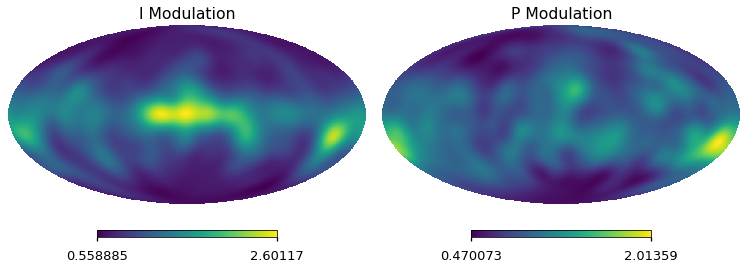
\includegraphics[width=2\columnwidth]{figures/mod_dust.png}\\
     
      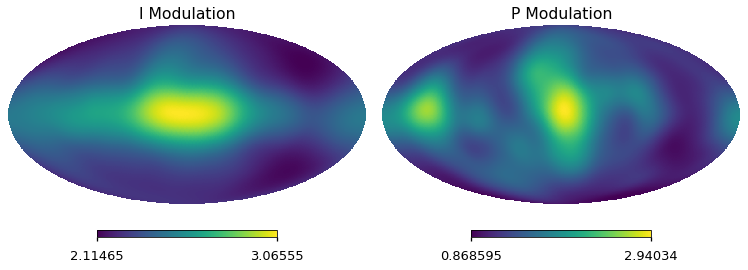
\includegraphics[width=2\columnwidth]{figures/mod_synch.png}\\
     \caption{Modulation maps for (top) dust and  (bottom) synchrotron. }
     \label{fig:modulation_maps }
 \end{figure*}
 

 
We remark here that the synthesis of small scales involves regions far from the Galactic plane.  We adopt the  \texttt{GAL097} \emph{Planck}  mask\footnote{\texttt{HFI\_Mask\_GalPlane-apo2\_2048\_R2.00.fits}} for dust . This is because, inside this area, the dust signal presents a very high SNR that small angular scales (e.g. $\sim20 $ arcmin ) are less affected by noise. We therefore decide to optimally exploit the state-of-art data on dust emission by employing the real small scales from observations nearby the Galactic plane.  

We follow a similar approach also for synchrotron and use the same mask as for dust to include real small scales in the Galactic plane region. Although synchrotron high-resolution data are currently lacking in this region, the inclusion of full resolution data, albeit coarser than the dust ones, surely encodes scales ($\sim 1$ deg) smaller   than   injection scale $\ell_1=38 $.  

To make the transition from the two regions piecewise, we make sure to apodize both masks have been apodized with a Gaussian profile with 5 deg length.



%\subsection{Dust emission}

%\subsubsection{Dust Amplitude}


%We first compute the $tt$, $ee$, and $bb$ power spectra from the dust template $i$, $q$, and $u$ maps and fit each with a power law $A\ell^{\gamma}$ in different multipole ranges depending on the native resolution of the map. Given that the intensity template has been estimated in a different way to the Q and U templates, we employ two different multipole scale cut-offs: $\ell=400$ and $100$, respectively. This further prevents the mixing of scales due to variable resolutions. Specifically, we employ $100 < \ell < 400$ for $tt$ and $30 < \ell < 110$ for $ee$ and $bb$. The spectral indices estimated from the fit are $\gamma = -1.29$, $-0.33$, and $-0.40$ for $tt$, $ee$, and $bb$, respectively.Adopting these values of $\gamma$ directly would lead to the $ee$ and $bb$ power exceeding $tt$ for large enough $\ell$ given the steeper index of the latter. {\bf Some words on why this is ok in principle but gives problems with polarization fraction in practice} We prevent this by adopting a common spectral index $\gamma = -1.29$ to extrapolate all three spectra to higher $\ell$. This choice is further motivated by the fact that the dust intensity template is provided at a higher resolution than the polarization ones, allowing to observe the dust specifics at higher detail with respect to the polarization data being more affected by noise and systematics. Although we are assuming that small scale polarized dust emission to be the same spectral index as the intensity one, this  is something that is physically intuitive and expected   from magneto-hydro dynamic simulations \citep[][]{Kim:2019}. We then generate $iqu$ maps encoding only small scales generated from the fit power law spectra and ranging from the pivot $\ell$-scale up to the multipole related to the desired pixel resolution scale of the dust map we want to simulate.  
%Since we want the small scales to be modulated by the amplitude of the dust emission at large scales, we apply two different modulations for the $i$ and for the $qu$ maps as they are convolved with different beam resolutions. We adopt  the $i$  map   smoothed at 5 deg as a template for both modulation maps.  We then identify a region encoding  low and intermediate Galactic latitudes by masking  all the pixels in the smoothed $i$ map  whose  value is $>4.5 \log ( \mu K )$.  The  intensity modulation is then constructed by performing two different normalization in the regions defined outside and inside  the mask. We use the \emph{MinMax} rescaling ranging   between $1$ and $2$ for the low-intermediate latitudes and between $0.1$ and $1$ for the high latitudes. For the polarization modulation map, we rescale similarly outside the mask between $0.1$ and $1$ but we saturate to   $1$  all the pixels  inside the low latitude region. Once the small scale maps are modulated, they are then co-added to the  low-pass filtered  $iqu$ maps (given the $\ell$-pivot scale) that encode  large scales only. Finally, the $iqu$ maps are transformed   back to the real $IQU$ maps  to perform the validation steps required to assess the quality of the maps. 



\subsubsection{Dust Spectral Parameters}
Smaller angular scales are also included for the dust spectral parameters, by means of extrapolating the power law fitted from the GNILC  maps of $\beta_d$ and $T_d$.  We employ a different procedure with respect to the one presented in Sect. \ref{subsec:methodology}.  
We consider the $I$ map smoothed  at 5 deg.  We then identify two  regions encoding  low and intermediate Galactic latitudes corresponding to the  \texttt{GAL080} \emph{Planck} mask.  The  intensity modulation is then constructed by performing two different normalization in the regions defined outside and inside  this mask.  We \emph{min-max} rescale the map in the area inside the mask so that it  ranges   between $1$ and $2$, whereas    between $0.1$ and $1$ for the high latitudes.

Moreover, we fit the power-law of the $\beta_d$ and $T_d$ power  spectra, in two different multipole ranges, respectively $200-400$ and $100-400$.  Since the fitted power law  indices are  flatter than the one employed for dust amplitudes  $\alpha_{\beta_d}= 0.04$ and $\alpha_{T_d} = -0.47$, we don't expect the  small scales to dominate when rescaling maps at lower and higher frequencies than the reference one ( 353 GHz). 


%\subsection{Synchrotron Emission}
 
\subsubsection{Synchrotron Spectral Parameters}\label{sec:beta_s}
 \textbf{Giuseppe:   } 
 We start from the $\beta_s$ map that has been already employed in the previous suite of PySM models \citet{Thorne:2017}. This map has been produced by combining data from WMAP and HASLAM \citep{mivilledeschenes:2008}. One of the most striking feature of this map is  the lack of information on sub-degree scales. This is an intrinsic limit of radio radio observations as   synchrotron emission  increases  with low frequencies.  However, \citet{Krachmalnicoff:2018} reported a study  on $\beta_s$ estimated from S-PASS data at $2.3 $ GHz and at $10'$ resolution.   Together with a higher level of spatial variations, the authors noted an increase in the variance with respect the one estimated in the $\beta_s$ map derived by \citet{mivilledeschenes:2008}.  In this work, we propose an improved  map of $\beta_s $, starting from the template from \citet{mivilledeschenes:2008} and also benefits of  the recent  S-PASS observations. In particular:  we subtract the offset term from $\beta_s$  and rescale the large scale $\beta_s$   map by a factor $1.572$ as proposed by \citet{Krachmalnicoff:2018}. We than fit a  power-law  in the multipole range  $2<\ell<38$ and estimated $\alpha_{\beta_s}=-0.61 $. We then synthesize  small scales  from the fitted power law,  and modulate them with a modulation map obtained from the intensity HASLAM template. Similarly to what we did for the dust, we  min-max rescaled the modulation map  between 0.1 and 1.1 in the region outside the \texttt{GAL080} mask and from 1.1 to 2 in the region inside. 
 Then we add the modulated small scale  and the  large scale maps, and we make sure also to sum  an offset around $-3.10$.
 
Finally, although small scales of $c_s$  have not been detected yet, we presumably expect as well sub-degree spatial variations for this synchrotron parameter. Small  scales at multipoles $\ell>36$  are therefore  included   assuming them to follow  the same power law as  the $\beta_s$ ones,  i.e. $\alpha _{c_s}=\alpha _{\beta_s} = -0.61$, and that are  modulated with the exact same modulation map as the one we  adopted for $\beta_s$.